As mentionned in the chapter introduction, this section presents results and figures from an article currently under review in Earth System Dynamics and included as a whole in the appendix. %todo:internal ref

Two coupled simulations were run with the ICOLMDZOR LAM, using the intermediate domain size ($R_{domain}=1500km$ and $NBP=60$). The setups are identical except for the inclusion of irrigation, and are referred to as \irr (with irrigation activated in ORCHIDEE) and \noirr (without irrigation). 
They were run for 13 years from 2010 to 2022, which enables capturing some interannual variability of the current climate, making the averages less sensitive to anomalies or biases from any single year or extreme event.

\subsection{Simulated irrigation}
\label{sec:irrig_eval}

%figure
\begin{figure}[htbp]
    \centering
    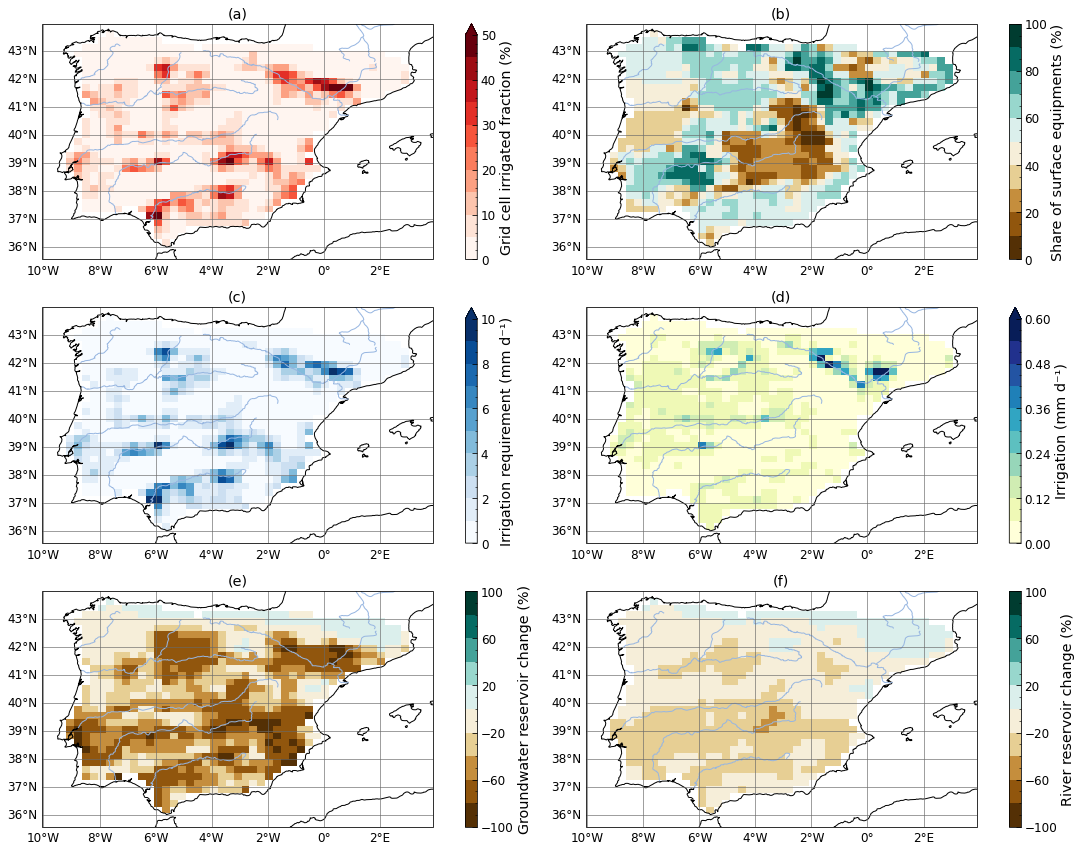
\includegraphics[width=\textwidth]{images/chap4/article/f03.png}
    \caption{Simulated irrigation and its drivers. Input maps of (a) grid cell irrigated fraction \citep[\% , derived from][]{hurtt_harmonization_2020} and (b) the share of irrigation equipment for surface withdrawals, as opposed to groundwater withdrawals \citep[\%, derived from ][]{siebert_groundwater_2010}. Annual means (2010-2022) of (c) simulated irrigation requirement (mm d$^{-1}$), (d) irrigation (mm d$^{-1}$), and relative changes (\irr - \noirr, \%) in water volumes in (e) groundwater and (f) river reservoirs.}
    \label{fig:irrig_maps}
\end{figure}

The computed irrigation demand (Fig. \ref{fig:irrig_maps}c) is highly dependent on the irrigated fraction (Fig. \ref{fig:irrig_maps}a) and much greater than the applied irrigation (Fig. \ref{fig:irrig_maps}d). This shows that irrigation is often constrained by water availability, with clear regional differences. Indeed, irrigation is much greater in the northern regions (Ebro and Douro river basins) than in southern regions (Guadiana and Guadalquivir basins) even though these regions have similar levels of irrigation demand (Fig. \ref{fig:irrig_maps}c, d).
As shown in Fig. \ref{fig:irrig_maps}b, southern regions (Guadalquivir Basin, upper Guadiana Basin) are more dependent on groundwater equipment for irrigation water withdrawals than the Ebro Basin, where withdrawals are taken mainly from surface water (overland and river reservoirs in the model).
Considering that the groundwater reservoir is much more depleted in the presence of irrigation than the river reservoir is (Fig. \ref{fig:irrig_maps}e, f), it is not surprising that the irrigation requirement cannot be met in these regions as much as it is in the north.
This depletion can be explained by the fact that the groundwater reservoir can only be filled with drainage in the grid cell, whereas the river reservoir can be fed from upstream grid cells and benefit from remote precipitation at the basin scale. It is also important to note that ORCHIDEE does not model deep groundwater storage, which is an important source of water for irrigation in southeastern Spain \citep{custodio_groundwater_2016}.

%figure : map of bias (irr vs obsEbro) + Seasonnal cycle over area with obs
\begin{figure}[htbp]
    \centering
    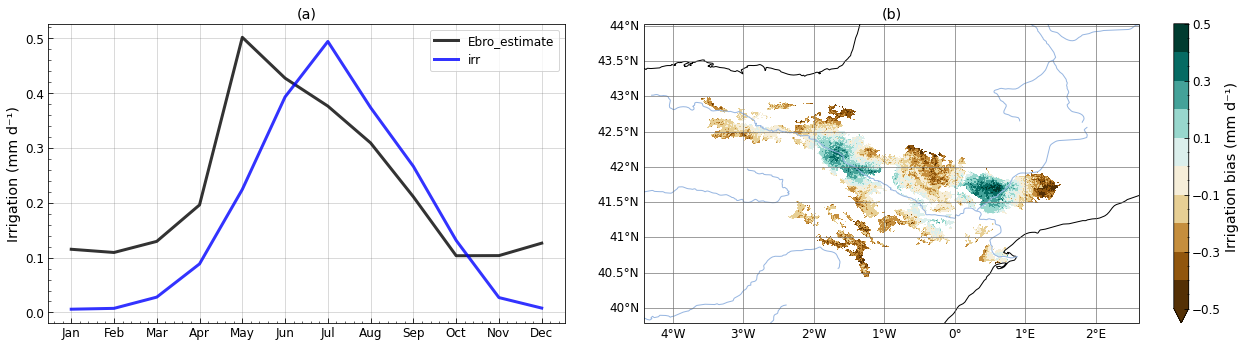
\includegraphics[width=\textwidth]{images/chap4/article/f04_horizontalized.png}
    \caption{Evaluation of simulated irrigation from January 2016 to July 2020 over the Ebro Valley. (a) Mean seasonal cycle of irrigation for the \irr simulation and the remote sensing product (\textit{Ebro\_estimate}, mm d$^{-1}$), and (b) mean bias compared with the product (mm d$^{-1}$). The simulation outputs are interpolated on the grid of the remote sensing product.}
    \label{fig:irrig_eval}
\end{figure}

In the Ebro Basin, simulated irrigation was evaluated using the irrigation remote sensing product from \cite{dari_regional_2023} with good overall performance, particularly in summer (Fig. \ref{fig:irrig_eval}a).
In winter, the model simulates almost no irrigation since it requires a minimum LAI to be activated, whereas the product shows irrigation all year long, which can be explained by the presence of winter crops not represented in the model.
A delay of the summer peak in the model compared with the product is noticeable, but the model might not be very far from actual irrigation since this product was found to be slightly ahead of actual irrigation based on benchmark volumes in some districts of the Ebro Valley \citep[Fig. 5 in ][]{dari_regional_2023}.
Spatially, the remote sensing product shows greater irrigation on the hillslopes than in the thalwegs, whereas the model simulates the opposite, with more intense irrigation next to the large rivers (Ebro, Segre, Cinca).
The resulting bias pattern (Fig. \ref{fig:irrig_eval}b) can be explained by the fact that in the model, water is mainly withdrawn from the river reservoir in this region, which is much greater in grid cells holding a large river than in upper areas of the valley. In reality, infrastructures such as the Canal d'Urgell in the Segre basin \citep{farran_urgell_2024}, enable gravity irrigation of hillslopes by diverting water from large rivers to neighbouring croplands. Including a representation of water adduction in the irrigation scheme by enabling withdrawal from adjacent grid cells could be a way to improve this bias.
Overall, the spatial biases of the simulated irrigation offset each other relatively well. Averaged over the subdomain where the satellite product provides values, the simulated irrigation is 0.20 mm d$^{-1}$ while the product estimates it at 0.23 mm d$^{-1}$.

\subsection{Impacts of irrigation on river discharge}
%todo:check que l'ajout des stations reste propre et cohérent

The simulated river discharge was evaluated against monthly data from 18 stations of the GRDC datbase (described in Section \ref{sec:eval_datasets}).
These stations, selected since they provided data over the simulation period and an had adequate position on the DEM grid, are described in Table \ref{table:stations_data} and shown in Fig. \ref{fig:selected_stations}. Most stations have available data from January 2010 to September 2017, and river discharge was therefore evaluated using the first eight years of simulation (2010-2017).

%figure:discharge stations and dams
\begin{figure}[htbp]
    \centering
    \includegraphics[width=\textwidth]{images/chap4/article/f02.pdf}
    \caption{Stations used for river discharge evaluation, river dams from \citet{aquastat_dams}, and main rivers of the study area from the CCM2.1 dataset \citep{vogt_pan-european_2007}, showing only rivers longer than 50 km for readability.}
    \label{fig:selected_stations}
\end{figure}

%table:description of discharge station used
\begin{table*}[htbp]
    \caption{Characteristics of river discharge stations used for evaluation. Stations marked with * are the largest of the five major basins of the Peninsula, and are shown in Fig. \ref{fig:discharge_SC}.
    }
    \resizebox{\textwidth}{!}{%
    \begin{tabular}{lcccccc}
        \toprule
        % \textbf{Station} & \textbf{Altitude (m)} & \textbf{River} & \textbf{Area (km²)} & \textbf{Mean discharge (m³/s)} & \textbf{Coverage (2010-2017, \%)} \\
        \textbf{Station} & \textbf{Altitude (m)} & \textbf{River} & \textbf{Area} & \textbf{Mean discharge} & \textbf{Coverage} \\
         & & & (km²) &  (m³/s) &  (2010-2017, \%) \\
        \midrule
        *1 (Tortosa)            & 25    & Ebro      & 84230     & 287.61 & 96.9 \\
        2 (Zaragoza)            & 189   & Ebro      & 40434     & 210.89 & 96.9 \\
        3 (Castejon)            & 265   & Ebro      & 25194     & 201.34 & 96.9 \\
        4 (Seros)               & 85    & Segre     & 12782     & 52.75  & 96.9 \\
        5 (Fraga)               & 100   & Cinca     & 9612      & 49.69  & 93.8 \\
        *6 (Tore)               & 637   & Douro     & 41808     & 109.18 & 96.9 \\
        7 (Peral De Arlanza)    & 766   & Arlanza   & 2413      & 16.44  & 96.9\\
        *8 (Talavera)           & 366   & Tagus     & 33849     & 46.77  & 34.4\\
        9 (Trillo)              & 727   & Tagus     & 3253      & 12.70  & 96.9 \\
        10 (Peralejos)          & 1143  & Tagus     & 410       & 3.87   & 96.9 \\
        *11 (Azud de Badajoz)   & 166   & Guadiana  & 48530     & 81.83  & 83.3 \\
        12 (Pulo do Lobo)       & 28    & Guadiana  & 61884     & 25.23  & 58.3 \\
        13 (La Cubeta)          & 758   & Guadiana  & 856       & 3.37   & 92.7 \\
        14 (Villarubia)         & 628   & Guadiana  & 10319     & 0.82   & 66.7 \\
        15 (Quintanar)          & 694   & Giguela   & 995       & 0.71   & 55.2 \\
        *16 (Mengibar)          & 240   & Guadalquivir & 16166  & 30.25  & 75.0 \\
        17 (Arroyo Maria)       & 538   & Guadalquivir & 583    & 6.19   & 86.5 \\
        18 (Pinos Puente)       & 561   & Frailes   & 357       & 1.00   & 87.5 \\
        \bottomrule
    \end{tabular}
    }
    \label{table:stations_data}
\end{table*}

%%single column figure : discharge obs vs irr vs no_irr on 3 stations (3 large rivers with proper data)
\begin{figure}[htbp]
    \centering
    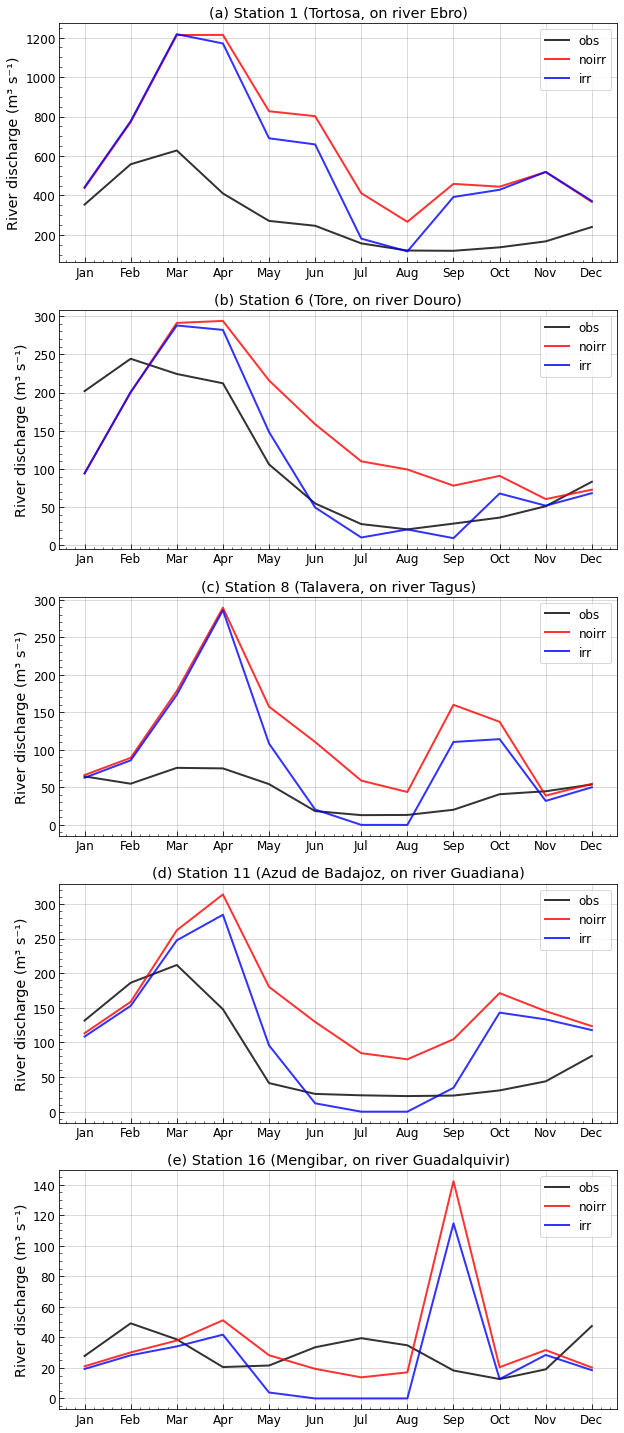
\includegraphics[width=8.3cm]{images/chap4/article/f05.png} 
    \caption{Impacts of irrigation on river discharge. Mean seasonal cycle of river discharge (m$^3$ s$^{-1}$) in observations (black) and the \noirr (red) and \irr (blue) simulations at five stations: (a) Tortosa (Ebro), (b) Tore (Douro), (c) Talavera (Tagus), (d) Azud de Badajoz (Guadiana), and (e) Mengibar (Guadalquivir). A mask is applied to the simulations to filter out months without corresponding observation data.}
    \label{fig:discharge_SC}
\end{figure}

Figure \ref{fig:discharge_SC} shows the average seasonal cycle of river discharge for the five largest rivers of the Peninsula (Ebro, Douro, Tagus, Guadiana, and Guadalquivir), for the two simulations and the GRDC observation data. The station with the greatest river discharge was selected for each river, to reflect integrated impacts of irrigation over the basin. A similar figure with all eighteen stations is presented in the appendix (Fig. \ref{fig:TS_discharge_18stations}, \ref{fig:TS_discharge_18stations}).
In most cases, the model shows a slight delay and a large overestimation of river discharge compared with observations, particularly in winter and spring. These errors can be related to the precipitation biases of the simulations, described in the next section, and to the lack of river dams in the model, which have a strong impact on actual discharge, given their high density in the Iberian Peninsula \citep[Fig. \ref{fig:selected_stations}, ][]{sabater_chapter_2022, moran-tejeda_reservoir_2012, lobera_geomorphic_2015}. In particular, the model overestimates the winter and spring discharge, a period when water is stored in dam reservoirs, which reduces the actual river flow.
The presence of dams also leads to unnatural seasonal cycles in the observations if river discharge is artificially increased in summer by the release of stored water (Fig. \ref{fig:discharge_SC}e).

The simulation of irrigation used cannot improve either of these aspects since it does not include a specific reservoir to store water. Its impact becomes noticeable in spring, with water withdrawals resulting in lower discharge during summer and autumn, generally leading to a much better match with observations (Fig. \ref{fig:discharge_SC}). 
As shown in Table \ref{table:stations_metrics}, for all fifteen stations where the mean bias is positive in the \noirr simulation, this bias is reduced in the presence of irrigation (in three cases it becomes negative but the absolute value is reduced). However, for the three stations where the \noirr bias is negative (n°10, 13, 17), it is worsened in the \irr simulation. On average, the \irr simulation exhibits clear improvements of the mean bias (-41.8 \%) and root mean square error (RMSE, -7.12 \%). The Pearson correlation coefficient is 0.56 on average in \noirr and is slightly improved (+0.02), with mostly small changes except for stations 6 and 8 (+0.09 and +0.08). Improvements are also observed for Nash-Sutcliffe efficiency (NSE, +0.67) and Kling-Gupta efficiency (KGE, +0.2), mostly as a consequence of improvements in the mean bias. However, only eight out of eighteen stations have a positive value of NSE and KGE values in the \noirr simulation (not shown), limiting the relevance of this average increase. In particular, the average NSE value is strongly influenced by a few stations (n°5, 8, 15) with initial NSE values below -10.

Overall, the performance is clearly improved for 12 stations but partly degraded for 6 stations, although three of them (n°10, 13, 17) have a very small average discharge. This may explain why small changes in the model can lead to large changes in performance and limits their relevance compared with larger stations. If only stations with an average annual discharge greater than 10 m³ s$^{-1}$ are considered, irrigation improves performance in nine out of twelve cases, and degrades it for three stations. One station (n°9) exhibits an unexpected increase in the spring discharge peak which originates mostly from a single year (2011, see Fig. \ref{fig:TS_discharge_18stations}) and worsens an already-existing 250 \% bias in this season. The other two (n°4 and 5) are close to the Pyrenees mountains and present very strong biases in both simulations (300 \% overestimation in spring, unexpected double peak in March and June, Fig. A2). These discrepancies are likely related to biases in precipitation (discussed hereafter) and were not positively impacted by irrigation, apart from the mean bias.

\begin{table*}[hbtp]
    \resizebox{\textwidth}{!}{
    \begin{tabular}{lccccccccc}
        \toprule
        \textbf{Station} & \textbf{Mean discharge} & \textbf{Bias} & \textbf{Bias} & \textbf{RMSE change} & \textbf{r change} & \textbf{NSE change} & \textbf{KGE change} \\
        & (\textit{obs}, m$^3$ s$^{-1}$) & (\noirr,  \%) & (\irr, \%)  & (\textit{irr - no\_irr}, \%) & (\textit{irr - no\_irr}) & (\textit{irr - no\_irr})  & (\textit{irr - no\_irr})  \\
        % \textbf{Station} & \textbf{Mean discharge (obs, m³/s)} & \textbf{Bias\\(\noirr, \%)} & \textbf{Bias\\Change (\%)} & \textbf{RMSE\\Change (\%)} & \textbf{r\\change} & \textbf{NSE\\change} & \textbf{KGE\\change} \\

        \midrule
        *1 (Tortosa)        & 287.61  & 126.3 & \textbf{103.4} & \textbf{-7.88} & \textbf{0.03}  & \textbf{0.56}  & \textbf{0.13}  \\
        2 (Zaragoza)        & 210.89  & 27.6 & \textbf{11.5}   & \textbf{-13.10}  & \textbf{0.01}  & \textbf{0.06}  & \textbf{0.10}  \\
        3 (Castejon)        & 201.34  & 30.7 & \textbf{21.4}   & \textbf{-1.45}  & \textbf{0.01}  & \textbf{0.01}  & \textbf{0.03}  \\
        4 (Seros)           & 52.75   & 240.3 & \textbf{227.7} & 0.81   & -0.02 & -0.54 & -0.09 \\
        5 (Fraga)           & 49.69   & 193.2 & \textbf{179.8} & 1.81   & -0.01 & -1.78 & -0.22 \\
        *6 (Tore)           & 109.18  & 36.9 & \textbf{-0.2}   & \textbf{-16.24} & \textbf{0.09}  & \textbf{0.21}  & \textbf{0.25}  \\
        7 (Peral De Arlanza) & 16.44  & 40.7 & \textbf{35.2}   & \textbf{-3.12}  & \textbf{0.01}  & \textbf{0.04}  & \textbf{0.04}  \\
        *8 (Talavera)       & 46.77   & 152.4 & \textbf{95.8}  & \textbf{-10.84} & \textbf{0.08}  & \textbf{2.29}  & \textbf{0.16}  \\
        9 (Trillo)          & 12.70   & 60.8 & \textbf{59.7}   & 0.76   & \textbf{0.03}  & -0.15 & -0.05 \\
        10 (Peralejos)      & 3.87    & -34.6 & -38            & 1.82   & \textbf{0.01}  & -0.03 & -0.01 \\
        *11 (Azud de Badajoz) & 81.83 & 90.5 & \textbf{34.3}   & \textbf{-14.26} & \textbf{0.05}  & \textbf{0.24}  & \textbf{0.51}  \\
        12 (Pulo do Lobo)   & 25.23   & 287.3 & \textbf{162.0} & \textbf{-18.53} & \textbf{0.03}  & \textbf{1.48}  & \textbf{1.17}  \\
        13 (La Cubeta)      & 3.37    & -10.7 & -36.2          & 5.82   & -0.01 & -0.12 & -0.12 \\
        14 (Villarubia)     & 0.82    & 152.4 & \textbf{61.0}  & \textbf{-3.53} & -0.03 & \textbf{0.29}  & \textbf{0.53}  \\
        15 (Quintanar)      & 0.71    & 312.7 & \textbf{149.3} & \textbf{-17.89} & 0.00  & \textbf{9.31}  & \textbf{0.98}  \\
        *16 (Mengibar)      & 30.25   & 19.4 & \textbf{-16.9}  & \textbf{-4.52} & \textbf{0.01}  & \textbf{0.46}  & \textbf{0.09}  \\
        17 (Arroyo Maria)   & 6.19    & -35.4 & -47.5 & 8.44   & -0.04 & -0.28 & -0.10 \\
        18 (Pinos Puente)   & 1.00    & 27.0 & \textbf{-3.0}   & \textbf{-5.59}  & \textbf{0.03}  & \textbf{0.06}  & \textbf{0.12}  \\
        \midrule
        Mean                & 63.37   & 95.4 & \textbf{55.5}   & \textbf{-7.12} & \textbf{0.02}  & \textbf{0.67}  & \textbf{0.20}  \\
        \bottomrule
    \end{tabular}
    }
    \caption{Station mean discharge (\textit{obs}, m$^3$ s$^{-1}$), discharge bias (for the \noirr and \irr simulations, in \%), and change in evaluated metrics (\irr - \noirr) for the RMSE (relative change in \%), Pearson correlation coefficient $r$, Nash-Sutcliffe efficiency and Kling-Gupta efficiency. Model performance improvements when using irrigation are shown in bold. Stations marked with * are the largest of the five major basins of the Peninsula, and are shown in Fig. \ref{fig:discharge_SC}.}
    \label{table:stations_metrics}
\end{table*}

% \clearpage

\subsection{Evaluation of precipitation and ET and influence of irrigation}

%figure: precip and ET eval, side by side Seasonal Cycle (with obs products) and bias to GPCC/GLEAM
\begin{figure}[htbp]
    \centering
    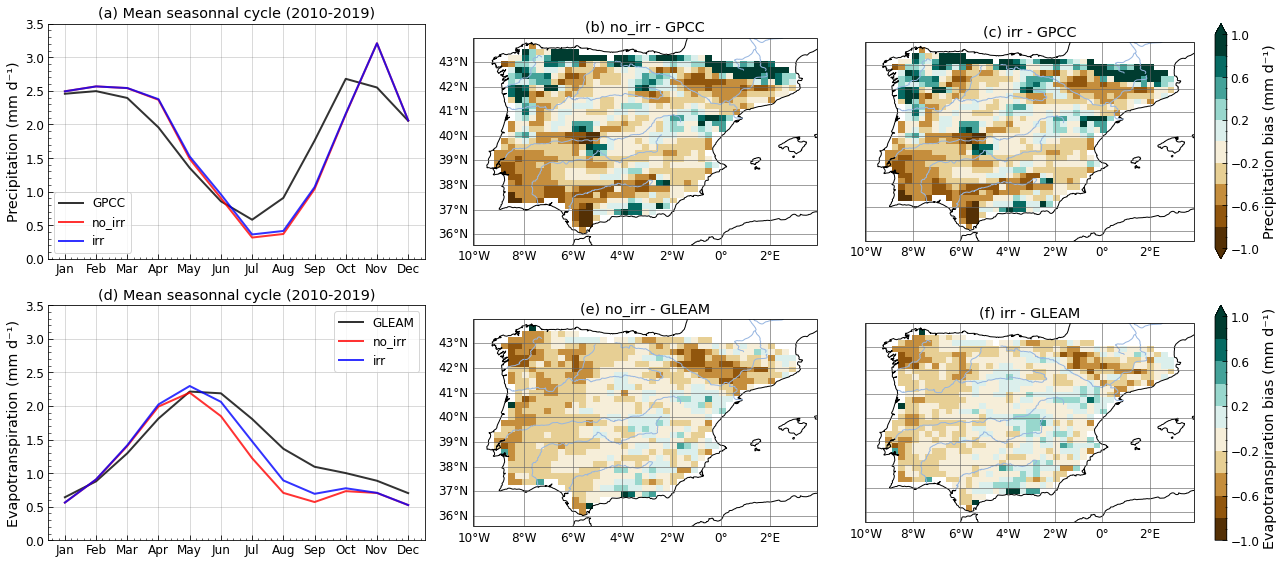
\includegraphics[width=\textwidth]{images/chap4/article/f06.png}
    \caption{Evaluation of simulated precipitation (P) and evapotranspiration (ET) over the Iberian Peninsula continental subdomain, from 2010 to 2019. 
    (a) Mean seasonal cycle of P (mm d$^{-1}$) for the two simulations and GPCC product, annual mean P bias of the (b) \noirr and (c) \irr simulations relative to the GPCC product (mm d$^{-1}$).
    (d) Mean seasonal cycle of ET (mm d$^{-1}$) for the two simulations and GLEAM4 product, annual mean ET bias of the (e) \noirr and (f) \irr simulations relative to the GLEAM4 product (mm d$^{-1}$).}
    \label{fig:sim_eval_ET_P}
\end{figure}

The simulated precipitation and ET were evaluated from 2010 to 2019 using the GPCC and GLEAM4 products, respectively (Fig. \ref{fig:sim_eval_ET_P}).
On average over the domain, the two simulations present very similar seasonal cycles of precipitation. The model is in good agreement with GPCC until June (Fig. \ref{fig:sim_eval_ET_P}a), but presents a strong underestimation of precipitation in summer, followed by a delayed and overestimated peak in autumn, which likely contributes to the biases of river discharge winter peaks visible in Fig. \ref{fig:discharge_SC}. 
This seasonal cycle is largely representative of the whole peninsula, although some spatial disparities persist. The two simulations exhibit very similar spatial patterns of annual mean precipitation, with a strong overestimation in elevated areas (Fig. \ref{fig:sim_eval_ET_P}b,c), which is a known bias of climate models \citep{arjdal_modeling_2024, adhikari_evaluation_2024}.
This is partly compensated by smaller underestimates of precipitation over large neighbouring areas, as seen in the Ebro Valley.

Both simulations match the GLEAM4 ET product well from January to May but underestimate ET for the rest of the year, particularly in summer (Fig. \ref{fig:sim_eval_ET_P}d). As expected, ET increases when irrigation is accounted for, particularly from May to September, which is the period where vegetation is the most developed and irrigation is the greatest. This partially alleviates the dry bias, but ET remains underestimated, even in the \irr simulation.
No similar patterns of biases between ET and incoming radiative fluxes were identified, and the remaining ET bias can be related to the underestimation of precipitation in the southwestern part of the Peninsula and in plains, such as the northern Ebro Valley (Fig. \ref{fig:sim_eval_ET_P}b, e). 
Along large rivers, the ET underestimation almost disappears in the \irr simulation (Fig. \ref{fig:sim_eval_ET_P}f). The increase in soil moisture due to irrigation directly translates into an increase in ET, corroborating the hypothesis that the region lies within the transition regime described by \citet{Budyko_1956}. 
In contrast, the ET bias remains significant in lightly irrigated grid cells such as hillslopes, which is consistent with the limits of simulated irrigation described in Section \ref{sec:irrig_eval} (Fig. \ref{fig:irrig_eval}).

\subsection{Atmospheric impacts of irrigation in summer}

\subsubsection{Statistical significance}
To assess the influence of irrigation on the model, a statistical significance test was used to filter out differences between the two simulations (\irr and \noirr) that may be the result of natural variability only. In Fig. \ref{fig:diff_sig_6vars}, a Student t-test is used to assess for each grid cell whether the mean difference between the two simulations  (\irr - \noirr) significantly differs from 0, with a p-value of 0.05 as the limit to reject the null hypothesis. Grid cells with nonsignificant changes are partly hidden with hatches.

\subsubsection{Results}
%figure : maps of JJA diff with non-sig grid cells hatched 
\begin{figure}[htbp]
    \centering
    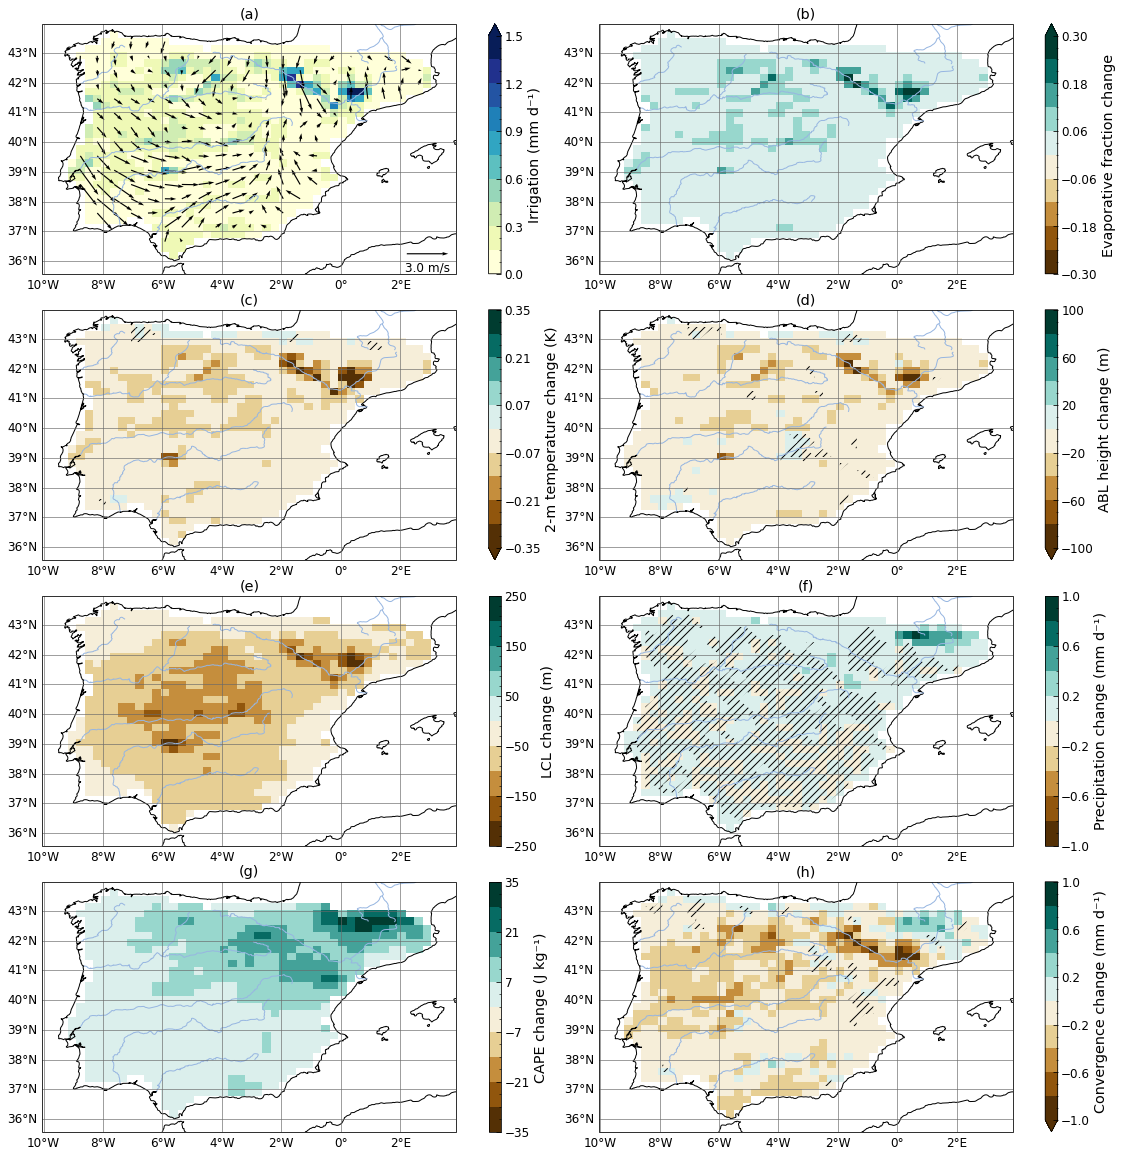
\includegraphics[width=15cm]{images/chap4/article/f07.png}
    \caption{Summer irrigation and its impacts (JJA, 2010-2022). (a) Irrigation (mm d$^{-1}$) and 10 m wind (\irr simulation). Mean changes in the presence of irrigation (\irr - \noirr): (b) evaporative fraction, (c) 2 m temperature (K), (d) atmospheric boundary layer height (m), (e) lifting condensation level (m), (f) precipitation (mm d$^{-1}$), (g) convective available potential energy (J kg$^{-1}$), (h) moisture convergence (mm d$^{-1}$). Hatching indicates areas where the change is not statistically significant.}
    \label{fig:diff_sig_6vars}
\end{figure}

The impacts of irrigation on atmospheric variables were studied with a focus on summer (JJA) since it is the season with the highest levels of simulated irrigation, with seasonal mean values of up to 1.5 mm d$^{-1}$ in the most intensely irrigated grid cells (Fig. \ref{fig:diff_sig_6vars}a).
In the presence of irrigation, the simulated latent heat flux ($LE$) increases across the entire Iberian Peninsula, by up to 50 W m$^{-2}$ in the Ebro Valley. As expected from the surface energy partitioning, this is compensated by a decrease in the sensible heat flux ($H$), which is almost equivalent in irrigated areas and leads to large increases in the evaporative fraction ($EF = \frac{LE}{LE+H}$) shown in Fig. \ref{fig:diff_sig_6vars}b.
When the sensible heat flux decreases, less energy is transmitted from the surface to the air, leading to a decrease in the 2-m air temperature which spatially matches the increase in $EF$. The order of magnitude remains low over most of the Peninsula, with the most important changes reaching -0.35 K in the Ebro Valley (Fig. \ref{fig:diff_sig_6vars}c).
The decreases in sensible heat flux and temperature also lead to a more stable boundary layer over most of the peninsula, but mostly in intensely irrigated areas where it is lowered by 100m (Fig. \ref{fig:diff_sig_6vars}d).
Moreover, the presence of irrigation results in a moister lower atmosphere, with an average specific humidity over the Peninsula increasing by 2.8 10$^{-4}$ kg kg$^{-1}$ in summer (+3.4 \%) and maximal local increases in the Ebro Valley of 1 10$^{-3}$ kg kg$^{-1}$ (+10 \%). Since air temperature changes in the atmospheric column are rather small, the lowering of the lifting condensation level (LCL) reflects this atmospheric moistening very well. It is most marked in the Ebro Valley, where the LCL is lowered by 250 m (-13 \%) in the most intensely irrigated grid cells, and remains significant even in areas where irrigation is low (Fig. \ref{fig:diff_sig_6vars}e).

The lowering of the ABL and LCL theoretically favour opposite effects on precipitation. On the one hand,  a lower and more stable ABL inhibits vertical mixing and convection, reducing the likelihood of cloud formation and deep convection initiation. On the other hand, if the LCL is lower, air parcels do not need to be lifted as high to condense, which increases the likelihood of cloud formation.
Over the most intensely irrigated areas, ABL stabilization seems to dominate and inhibit convective development since no significant change in precipitation is observed.
However, mountainous areas surrounding the Ebro Valley show significant increases in precipitation (Fig. \ref{fig:diff_sig_6vars}f). This can be understood because ABL stabilization remains weak in these zones whereas humidity can still be increased if moisture is advected (Fig. \ref{fig:diff_sig_6vars}d, e). In particular, the dominant wind patterns in the Ebro Valley (Fig. \ref{fig:diff_sig_6vars}a) indicate that the additional atmospheric moisture from irrigated areas is driven towards the valley slopes, which is consistent with the increases in moisture convergence (Fig. \ref{fig:diff_sig_6vars}h) and precipitation over the Pyrenees.
The competing interactions of ABL stabilization and atmospheric moistening are reflected by the increases in convective available potential energy (CAPE) which are most important in elevated areas around the valley (Fig. \ref{fig:diff_sig_6vars}g), where increases in precipitation are significant. 

% \clearpage

\subsection{Atmospheric moisture recycling over the Iberian Peninsula}
On average over the continental domain, the monthly change in ET in the presence of irrigation is well correlated with the amount of water added by irrigation and even exceeds it, particularly in summer months (the orange JJA data points in Fig. \ref{fig:scatter_IP}a are all on or above the 1:1 line).
In the simulation, ET is constrained by available water, and almost all the water added by irrigation is evaporated or transpired, meaning that this additional increase in ET comes from an additional input of water into the soil.
This is explained by a systematic increase in precipitation over the domain (all the data points are on or above the x-axis on Fig. \ref{fig:scatter_IP}b). This increase is also roughly proportional to the amount of applied irrigation, although the correlation is weaker than that for the increase in ET, and its values remain lower than the amount of water added by irrigation.
Therefore, it appears that irrigation contributes to an increase in atmospheric moisture, and that a part of this moisture is recycled as continental precipitation, which can then be reevaporated.

%figure: 2 scatter plots over IP domain, rainDiff vs irrig
\begin{figure}[htbp]
    \centering
    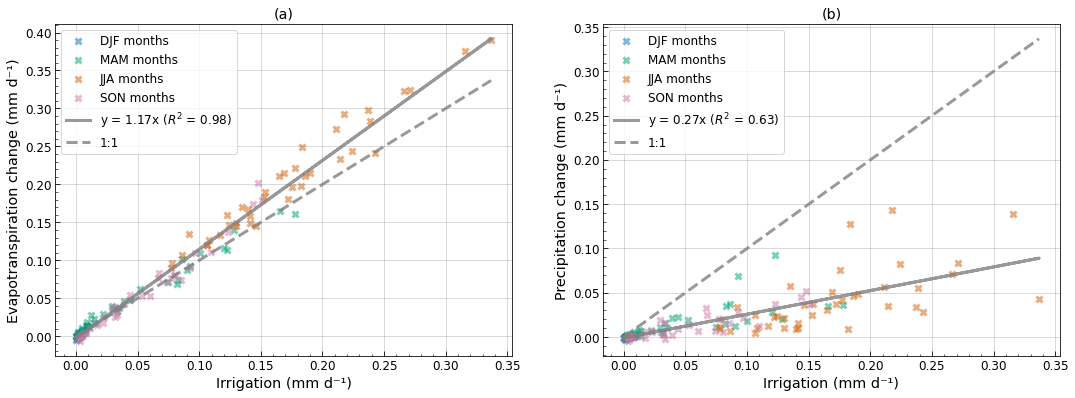
\includegraphics[width=\textwidth]{images/chap4/article/f08_colorblind.png}
    \caption{Domain-averaged influence of irrigation on monthly changes in ET and P (2010-2022). Each data point corresponds to the average value over the Iberian Peninsula continental domain for a single month of simulation (156 data points for 12 months over 13 years). The average amount of water added by irrigation in the \irr simulation (mm d$^{-1}$) is plotted against the average change (\textit{irr - no\_irr}) in (a) ET (mm d$^{-1}$) and (b) P (mm d$^{-1}$). The data points for the winter months are all concentrated around (0,0) for both figures because of very small irrigation volumes and changes in ET and P during this season.}
    \label{fig:scatter_IP}
\end{figure}

To look further into this recycling, three subdomains were defined, namely, low, medium and high irrigation areas, on the basis of the mean irrigation thresholds given in Table \ref{tab:irrig_lvl_areas}. In the map of simulated irrigation (Fig. \ref{fig:irrig_maps}d), the low irrigation domain corresponds to the first colour bin (yellow), the medium irrigation domain to the second bin (light green), and the high irrigation domain to the eight other bins. The three subdomains are also shown distinctly in Fig. \ref{fig:moisture_budget_annual}e.
On average, the increase in ET is slightly superior to irrigation for each subdomain (Fig. \ref{fig:moisture_budget_annual}).
However, the increase in precipitation is more than twice as large for the low irrigation subdomain than for the medium and high irrigation subdomains. Since irrigated areas are mostly in plains and valleys, this result is consistent with the increase in precipitation already described over mountainous areas in summer (Fig. \ref{fig:diff_sig_6vars}f). It points towards a nonlocal moisture recycling, with atmospheric moisture transfer from intensely irrigated areas to neighbouring lightly irrigated areas, meaning that a significant part of the additional rainfall does not occur on irrigated crops.
Over the entire Iberian Peninsula, the increase in precipitation represents 25 \% of the irrigated volume, whereas the increase in ET amounts to 112 \% of irrigation.

%t
% \begin{table}[t]
\begin{table}[h]
        \begin{tabular}{lcccc}
            \toprule
            \textbf{Subdomain} & \textbf{Areal fraction} & \textbf{Min. irrigation} & \textbf{Max. irrigation} & \textbf{Mean irrigation}\\
            & (\% of Iberian Peninsula) & (mm d$^{-1}$) & (mm d$^{-1}$) & (mm d$^{-1}$)\\
            \midrule
            Low irrigation      & 56.3    & 0.0   & 0.06  & 0.033 \\
            \midrule
            Medium irrigation   &  34.0   & 0.06  & 0.12  & 0.082\\
            \midrule
            High irrigation     &  9.7   & 0.12  & 0.61  & 0.210\\
            \bottomrule
        \end{tabular}
    \label{tab:irrig_lvl_areas}
    \caption{Subdomains of different irrigation intensity.}
\end{table}

%figure: moisture budget : barplot for 3 zones +IP
\begin{figure}[htbp]
    \centering
    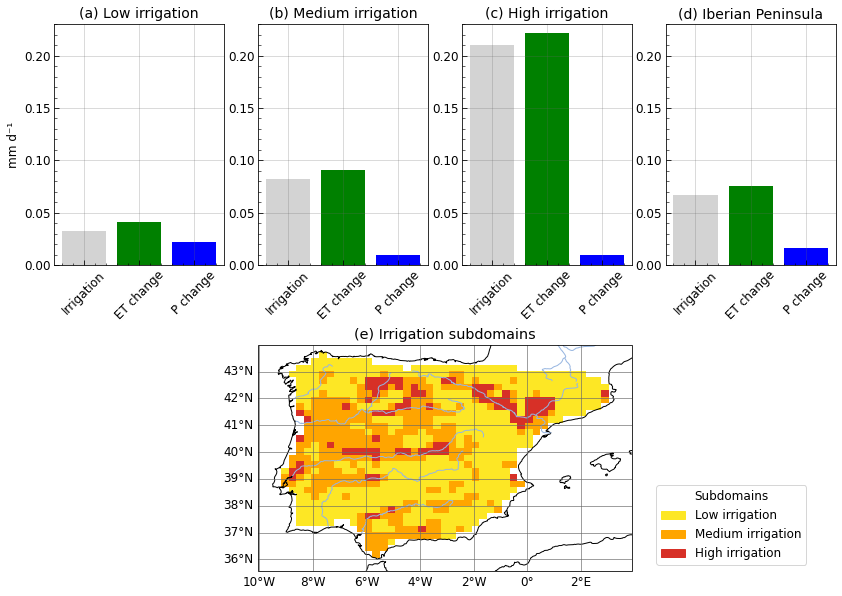
\includegraphics[width=12cm]{images/chap4/article/f09.png}
    \caption{Changes in the atmospheric moisture budget for subdomains with different irrigation intensities. Each bar plot shows the annual mean irrigation in the \irr simulation (2010-2022, mm d$^{-1}$) alongside the changes (\textit{irr - no\_irr}) in ET (mm d$^{-1}$) and P (mm d$^{-1}$) averaged over distinct subsets of the domain: (a) low irrigation, grid cells with an annual average irrigation lower than 0.06 mm d$^{-1}$, (b) medium irrigation, those where it is between 0.06 and 0.12 mm d$^{-1}$, (c) high irrigation those where it is higher than 0.12 mm d$^{-1}$, and (d) the Iberian Peninsula includes all 3 subsets. The three subdomains are shown in (e).}
    \label{fig:moisture_budget_annual}
\end{figure}

\clearpage
